\documentclass[journal, a4paper]{IEEEtran}

\usepackage{graphicx}
\usepackage{url}
\usepackage{amsmath} 
\usepackage{subcaption}

\begin{document}

	\title{Assignment III\\Boosting and Gaussian Processes}
	\author{Adam Kosiorek}	
	\markboth{Machine Learning for Applications in Computer Vision, Institute of Computer Vision, Technische Universit\'at M\"unchen}{}
	\maketitle
	
	
\section{Objective}
    \PARstart{T}{he} aim of the third assignment was to get insight into workings of Boosting and Gaussian Process (GP) algorithms by comparing performance and estimating uncertainty of several variants of the algorithms.
    
\section{Dataset}
    Boosting algorithms were compared on the MNIST dataset, which is comprised of 60000 training and 10000 testing samples \cite{MNIST}. Each sample is a 28x28 pixel black and white image of a single centered digit. It is widely used as a benchmark for comparing machine learning algorithms. 
    
    GPs were evaluated on an artificial 2-class dataset. It was randomly generated from a Gaussian distribution with expected values and covariance matrices as denoted by $\bar{x}$ and $\Sigma$ in equations \ref{eq:mean} and \ref{eq:cov}.
    
    \begin{equation}
     \bar{x}_{positive} = \begin{pmatrix} 0.75 \\ 0 \end{pmatrix} \;\; 
     \bar{x}_{negative} = \begin{pmatrix} -0.75 \\ 0 \end{pmatrix}
     \label{eq:mean}
    \end{equation}
    \begin{equation}
     \Sigma_{positive} = \begin{pmatrix} 1 & 0 \\ 0 & 1 \end{pmatrix} \;\; 
     \Sigma_{negative} = \begin{pmatrix} 1 & 0.95 \\ 0.95 & 1 \end{pmatrix}
     \label{eq:cov}
    \end{equation}

    
    \begin{figure}[ht]      
      \begin{subfigure}{.22\textwidth}
	\centering
	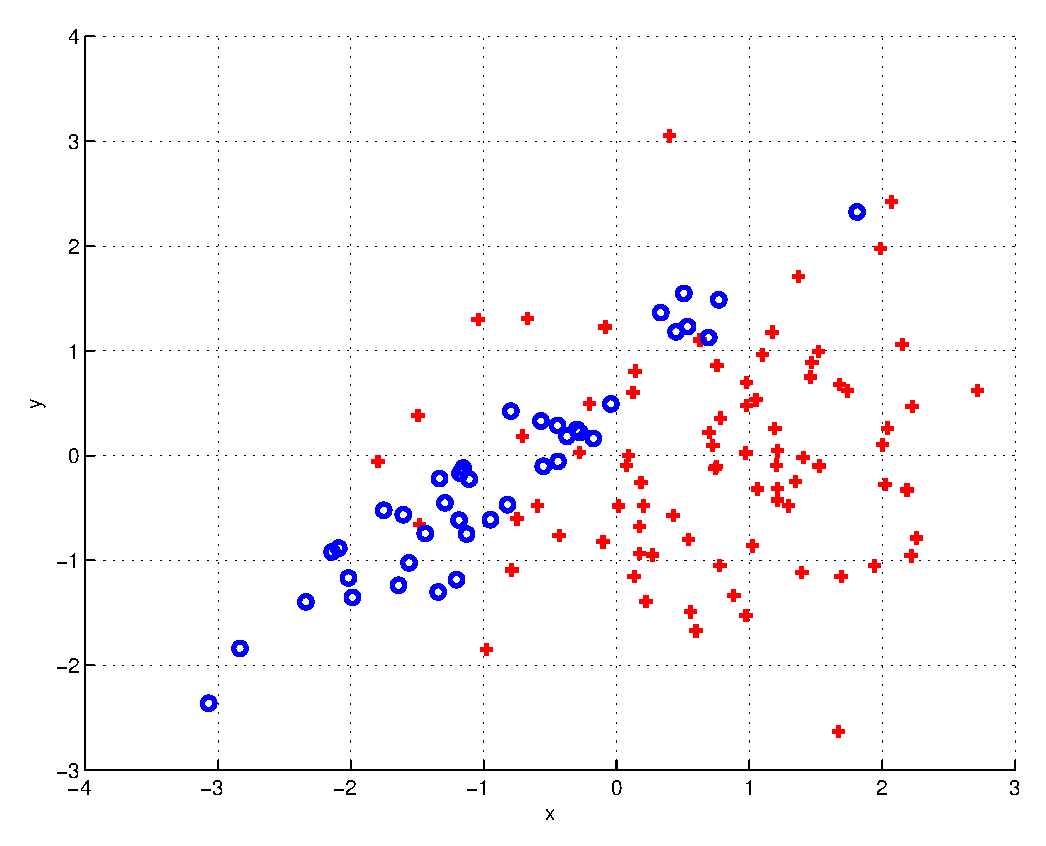
\includegraphics[width=.9\linewidth]{GP_trainset}
	\caption{}
	\label{fig:GP_a}
      \end{subfigure}
      \begin{subfigure}{.22\textwidth}
	\centering
	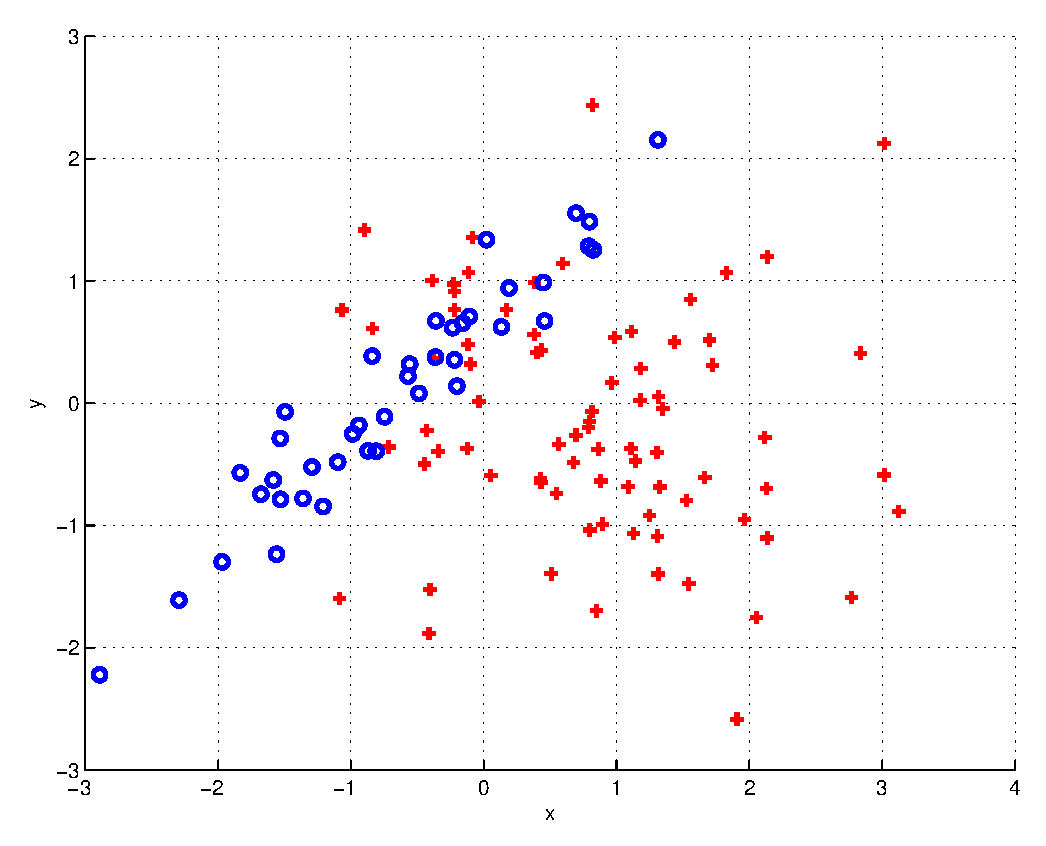
\includegraphics[width=.9\linewidth]{GP_testset}
	\caption{}
	\label{fig:GP_b}
      \end{subfigure}    
    
      \caption{(a) trainset and (b) testset for GPs. \textbf{+} denotes positive samples and \textbf{o} denotes negative samples.}
      \label{fig:GP_data}      
    \end{figure}

\section{Methods}
    Boosting is a means of combining weak classifiers, that is, classifiers only slightly better than random classifiers, in order to create a strong classifier. It does so by sequentially minimizing an exponential loss function by adding parameterized basis functions to the growing ensemble of weak classifiers. Here, a basis function means any weak classifier capable of handling weighted data, \textit{e.g.} decision trees or decision stumps.
    
    Gaussian Process is a collection of random variables, any finite number of which have a joint Gaussian distribution. Since the number of variables can be infinite, a Gaussian Distribution is a distribution over functions. Therefore, if we have a mean function and covariance function, we can sample from the Gaussian Process. The infinite number of variables can be handled due to marginalization property, which allows operation on finite vectors only.

\section {Experiments and Results}
  All experiments were carried out on raw data (without any preprocessing) on a notebook with Intel i7-2670QM quad core CPU and 8GB RAM in Matlab using Matlab Boosting Framework \cite{MATLAB_BOOST} and Gaussian Processes for Machine Learning (GPML) toolboxes \cite{GPML}. Assignment code is available on GitHub \cite{code}.
  
  \subsection{Boosting}
      I compare AdaBoost, RUSBoost, LPBoost and TotalBoost algorithms trained and tested on small part of the dataset (1000 training and testing samples) and full dataset with different ensemble sizes. The ensemble size is a hyper-parameter for the first two algorithms and it is automatically chosen for the last two due to the self-termination property. LPBoost terminated with 128 and 6 classifiers, while TotalBoost terminated with 28 and 51 classifiers when trained on 1000 samples and on the whole dataset respectively. AdaBoost significantly outperforms all other algorithms. According to \cite{MATLAB_BOOST} TotalBoost and LPBoost are ill-suited for problems with large number of observations, which is the case here, while RUSBoost is especially effective for unbalanced data classification problems. Obviously, an increased size of the training set as well as an increased number of weak classifiers positively impacts the classification accuracy.
  
    \begin{figure}[ht]    
      \centering
      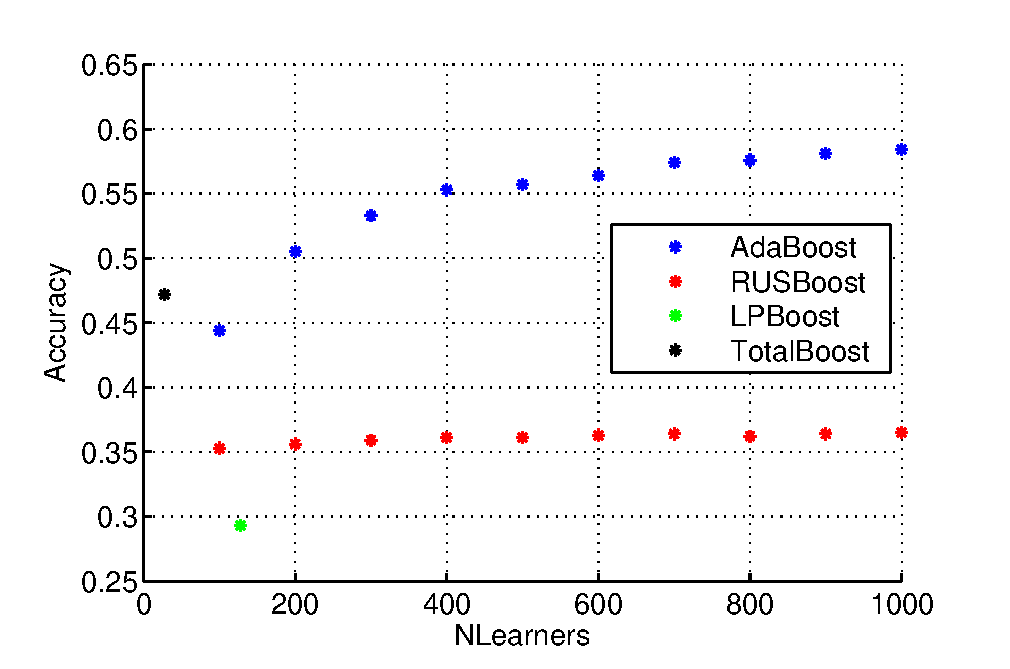
\includegraphics[width=\linewidth]{boost_plot_small}
      \caption{Classification accuracy of Boosting classifiers trained and tested on 1000 samples.}
      \label{fig:boost_accuracy_small}
    \end{figure}
    
    \begin{figure}[ht]    
      \centering
      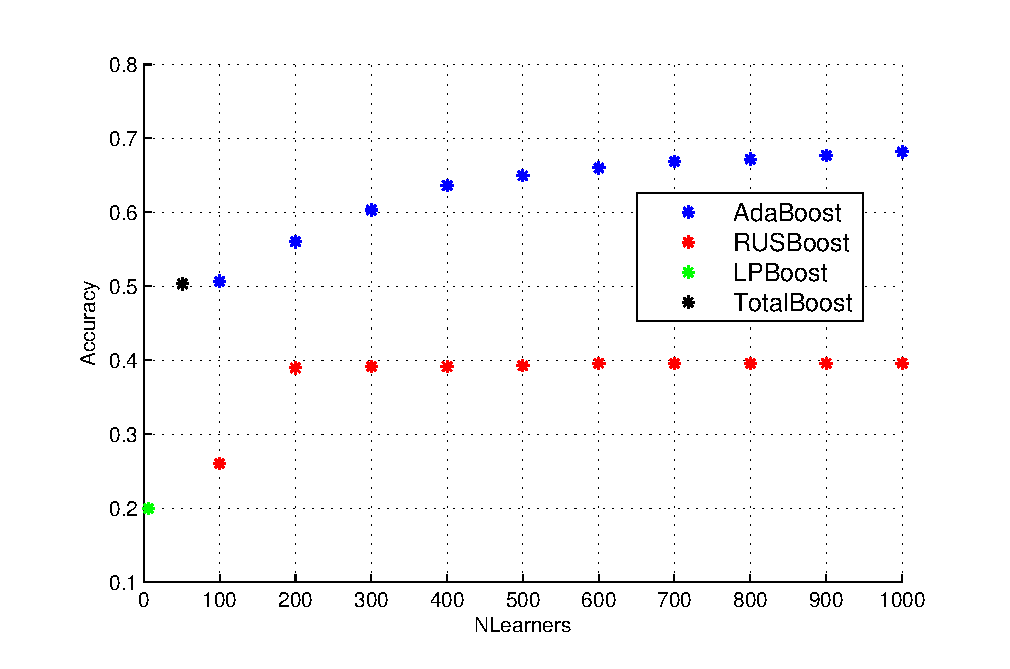
\includegraphics[width=\linewidth]{boost_plot_big}
      \caption{Classification accuracy of Boosting classifiers trained and tested on the whole dataset.}
      \label{fig:boost_accuracy_big}
    \end{figure}
    
    Figures \ref{fig:boost_true} and \ref{fig:boost_false} show classification uncertainty histograms for AdaBoost with 1000 weak classifiers and 10000 test samples. Both histograms resemble a Gaussian distribution. Boosting classifiers ouput scores instead of probabilities in Matlab and they had to be normalized before entropy could be computed. Since it is a multi-class classification problem, I used the following formula for computing classification entropy:
    
    \begin{equation}
      h = -\Sigma_{c=1}^C p_c * log(p_c)
    \end{equation}
    
    
     \begin{figure}[ht]
      \centering
      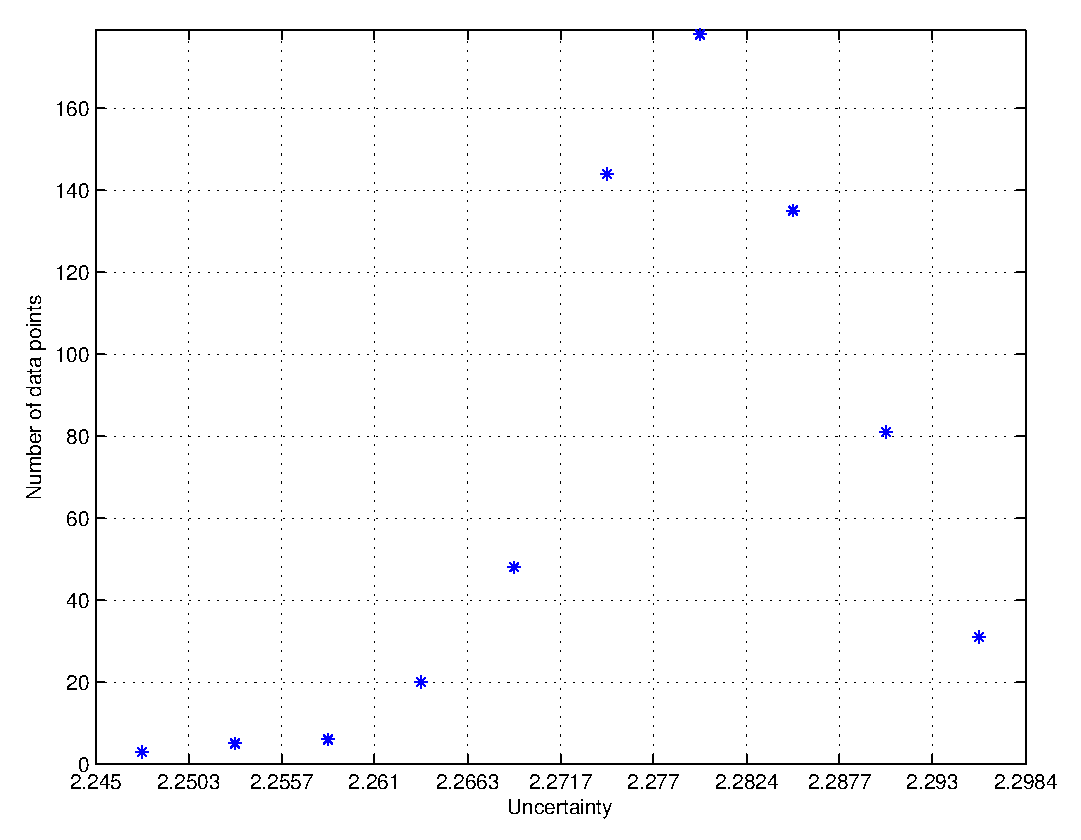
\includegraphics[width=.8\linewidth]{ada_correct}
      \caption{AdaBoost classification uncertainty histogram for correctly classified test samples.}
      \label{fig:boost_true}
    \end{figure}

    \begin{figure}[ht]
      \centering
      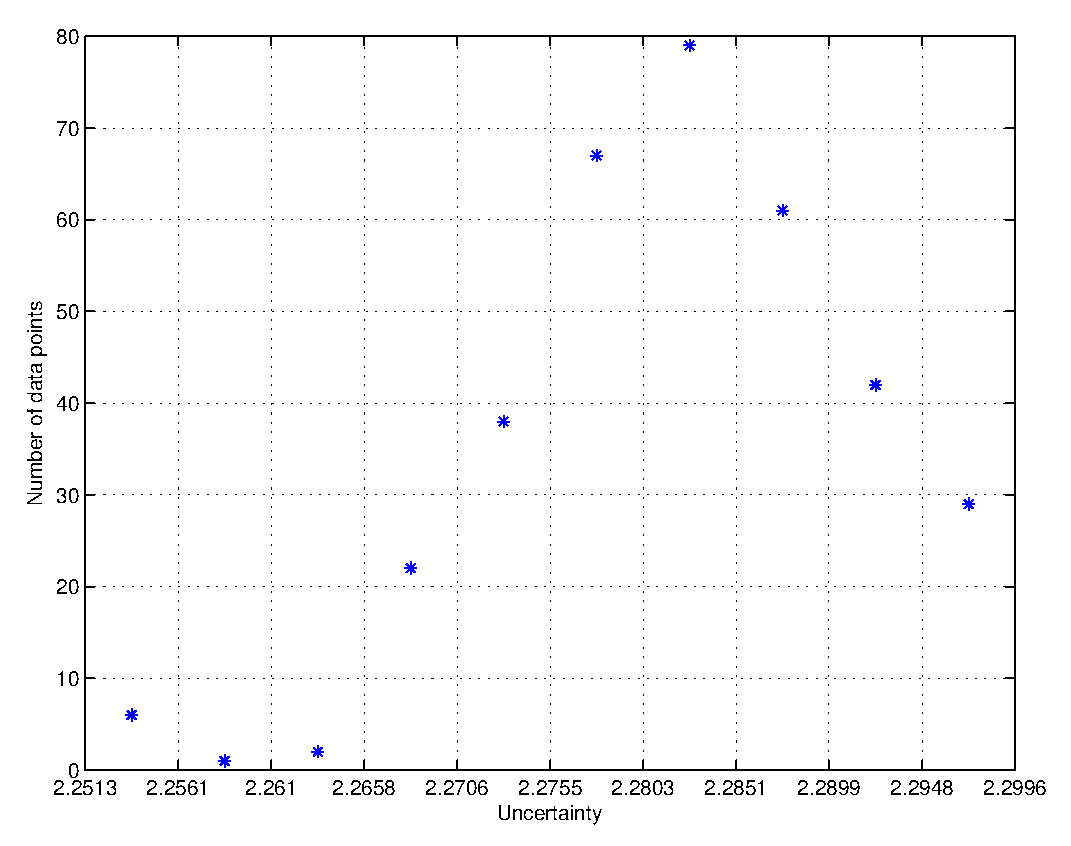
\includegraphics[width=.8\linewidth]{ada_incorrect}
      \caption{AdaBoost classification uncertainty histogram for incorrectly classified test samples.}
      \label{fig:boost_false}
    \end{figure}
    

    
   
  \subsection{Gaussian Processes}
      GPs output log probabilities instead of class labels. To compute accuracy and uncertainty I have taken the exponent of the log probability and thresholded it with a value of $0.5$, taking class label $l=1$ for probabilities greater than the threshold value and $l=-1$ for probabilities smaller than the threshold value. Table \ref{tab:GP_acc} shows accuracy of GPs with different covariance, likelihood and inference functions, while figures \ref{fig:GP_true} and \ref{fig:GP_false} depict uncertainty histograms for one of the GP variants with the highest accuracy, namely with linear isotropic (LINiso) covariance function.
      
      
    \begin{table}[ht]
      \begin{center}
	\caption{GP accuracy}
	\label{tab:GP_acc}
	\begin{tabular}{c|c|c|c}
	  covariance & likelihood  & inference  & accuracy \\ \hline
	  SEard & Erf & EP & 0.62\\ \hline
	  SEiso & Erf & EP & 0.63\\ \hline
	  LINard & Erf & EP & 0.68\\ \hline
	  LINard & Gaus & Exact & 0.55\\ \hline
	  LINard & Logistic & EP & 0.68\\ \hline
	  LINiso & Erf & EP & 0.68
	\end{tabular}
      \end{center}
    \end{table}

    \begin{figure}[ht]
      \centering
      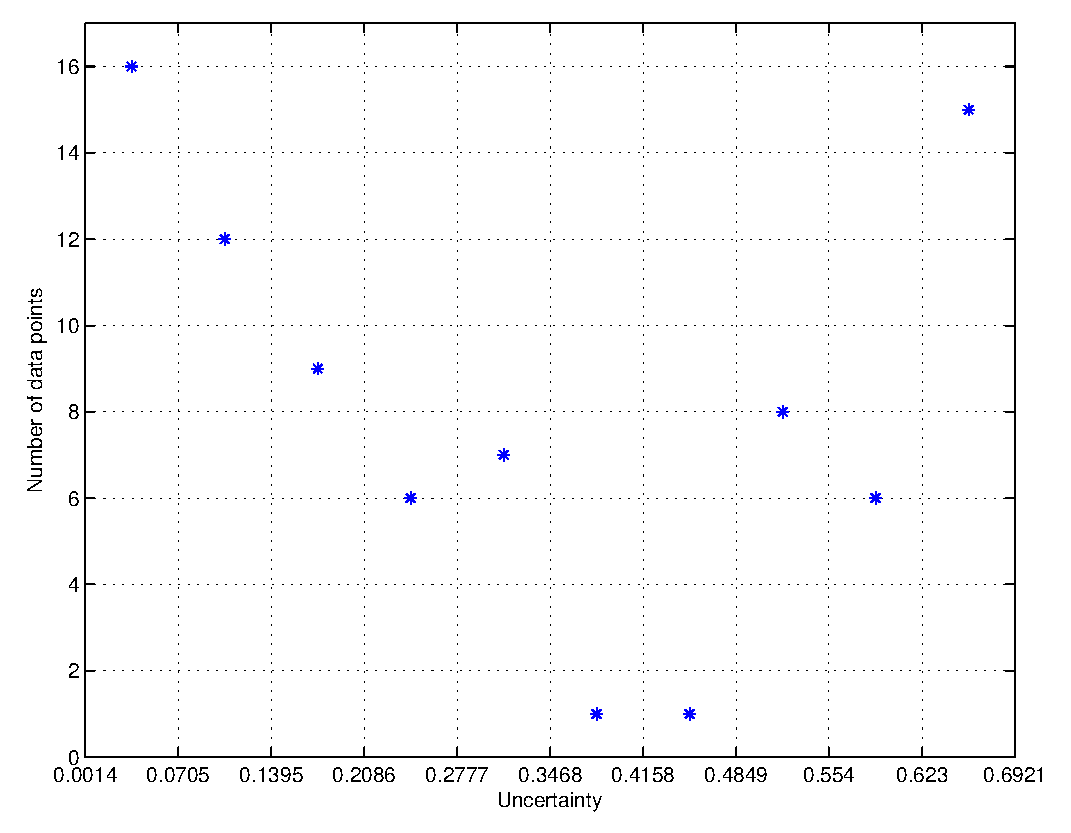
\includegraphics[width=.8\linewidth]{covLINiso_likErf_infEP_true}
      \caption{GP classification uncertainty histogram for correctly classified test samples.}
      \label{fig:GP_true}
    \end{figure}

    \begin{figure}[ht]
      \centering
      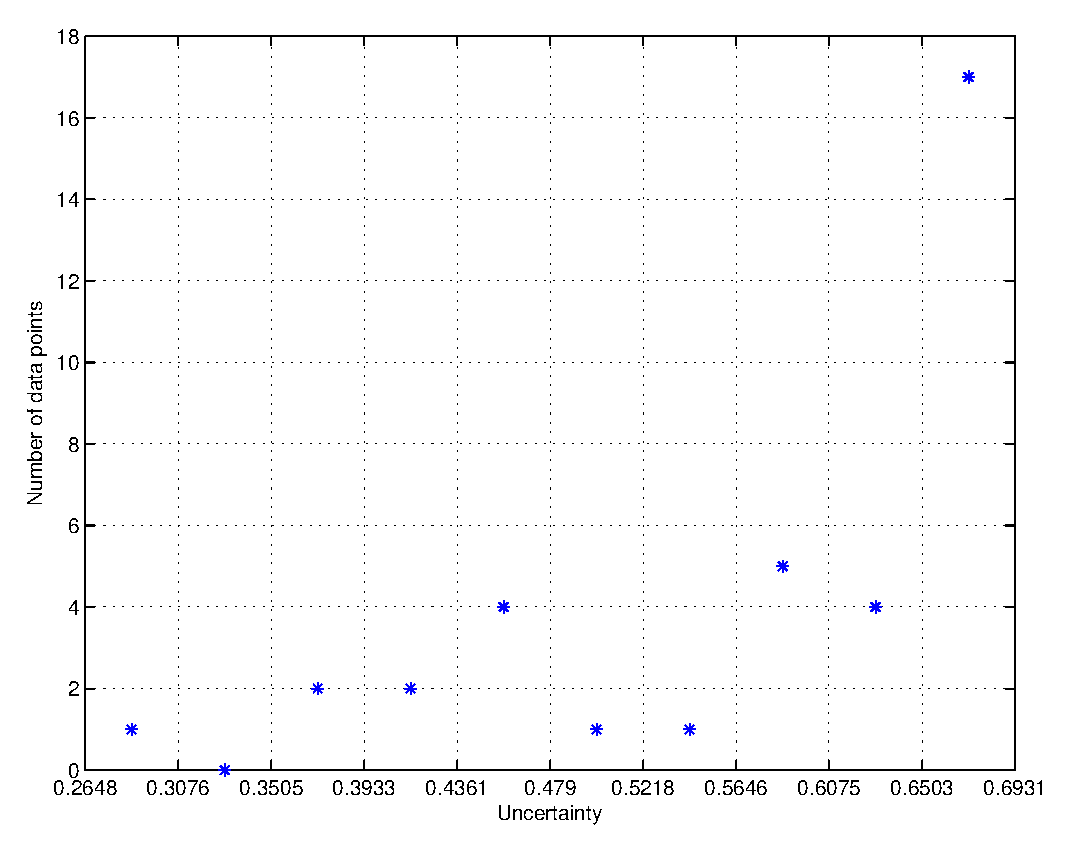
\includegraphics[width=.8\linewidth]{covLINiso_likErf_infEP_false}
      \caption{GP classification uncertainty histogram for incorrectly classified test samples.}
      \label{fig:GP_false}
    \end{figure}    
  \subsection{Discussion}


%   \begin{figure}[h]    
%     \centering
%     \includegraphics[width=.8\linewidth]{}
%     \caption{Images for Classification.}
%     \label{fig:imgs}
%   \end{figure}
% 
% 
%   \begin{table}[h]
%     \begin{center}
%     \caption{Classification Results}
%     \label{tab:results}
%     \begin{tabular}{c|c|c|c|c}
%       \# & \#class  & class name  & probability & entropy \\ \hline
%       a & 428 & barrow, garden cart, lawn cart, \ldots & 0.07 & 5.22\\ \hline
%       b & 311 & grasshopper, hopper & 0.14 & 3.72\\ \hline
%       c & 403 & aircraft carrier, carrier, flattop, \ldots & 0.13 & 4.67\\ \hline
%       d & 620 & laptop, laptop computer & 0.12 & 4.63\\ \hline
%       e & 673 & mouse, computer mouse & 0.41 & 2.75\\ \hline
%       f & 947 & mushroom & 0.76 & 1.17\\ \hline
%       g & 834 & suit, suit of clothes & 0.62 & 1.09\\ \hline
%       h & 980 & volcano & 0.36 & 3.32
%     \end{tabular}
%     \end{center}
%   \end{table}


\begin{thebibliography}{5}

    \bibitem{code}
    Assignment Code: \url{https://github.com/akosiorek/CSE/tree/master/MLCV/ex3/}

    \bibitem{MNIST}
    Y.~LeCun, L.~Bottou, Y.~Bengio, and P.~Haffner. ``Gradient-based learning applied to document recognition.'' Proceedings of the IEEE, 86(11):2278-2324, November 1998.

    \bibitem{GPML}
    C.~E.~Rasmussen and H.~Nickisch, ``Gaussian processes for machine learning (GPML) toolbox'', The Journal of Machine Learning Research, 2010, 11, 3011-3015.
    
    \bibitem{MATLAB_BOOST}
    Matlab Boosting Framework: \url{http://www.mathworks.com/help/stats/ensemble-methods.html}    
    

\end{thebibliography}

% Your document ends here!
\end{document}
